
%%%%%%%%%%%%%%%%%%%%%%% file typeinst.tex %%%%%%%%%%%%%%%%%%%%%%%%%
%
% This is the LaTeX source for the instructions to authors using
% the LaTeX document class 'llncs.cls' for contributions to
% the Lecture Notes in Computer Sciences series.
% http://www.springer.com/lncs       Springer Heidelberg 2006/05/04
%
% It may be used as a template for your own input - copy it
% to a new file with a new name and use it as the basis
% for your article.
%
% NB: the document class 'llncs' has its own and detailed documentation, see
% ftp://ftp.springer.de/data/pubftp/pub/tex/latex/llncs/latex2e/llncsdoc.pdf
%
%%%%%%%%%%%%%%%%%%%%%%%%%%%%%%%%%%%%%%%%%%%%%%%%%%%%%%%%%%%%%%%%%%%


\documentclass[runningheads,a4paper]{llncs}

\usepackage{amssymb}
\setcounter{tocdepth}{3}
\usepackage{graphicx}

\usepackage{url}
\urldef{\mailsa}\path|{alfred.hofmann, ursula.barth, ingrid.haas, frank.holzwarth,|
\urldef{\mailsb}\path|anna.kramer, leonie.kunz, christine.reiss, nicole.sator,|
\urldef{\mailsc}\path|erika.siebert-cole, peter.strasser, lncs}@springer.com|
\newcommand{\keywords}[1]{\par\addvspace\baselineskip
\noindent\keywordname\enspace\ignorespaces#1}
\def\boxend{\hspace*{\fill} $\Box$}
\newcommand{\comment}[1]{}

\begin{document}

\mainmatter

\title{\emph{TeenChat}: A Chatterbot System for Sensing and Releasing Adolescents' Stress}
\author{Jing Huang, Qi Li, Yuanyuan Xue, Taoran Cheng, Shuangqing Xu, \\Jia Jia, Ling Feng}
\institute{Dept. of Computer Science and Technology, Tsinghua University, Beijing, China \\
\{j-huang14,liqi13,xue-yy12,ctr10,xsq10\}@mails.tsinghua.edu.cn,
\{jjia,fengling\}@mail.tsinghua.edu.cn}
\maketitle
\begin{abstract}
More and more adolescents today are suffering from various adolescent stress.
Too much stress will bring a variety of physical and psychological problems
including anxiety, depression, and even suicide to the growing youths, whose
outlook on life and problem-solving ability are still immature enough.
Traditional face-to-face stress detection and relief methods do not work, confronted with adolescents who are reluctant
to express their negative emotions to the people in real life.
In this paper, we present a adolescent-oriented intelligent chatting system called \emph{TeenChat}, which acts as a virtual friend
to listen, understand, comfort, encourage, and guide stressful adolescents to pour out their bad feelings, and
thus releasing the stress. Our 1-month user study demonstrates \emph{TeenChat} is effective on sensing and helping adolescents' stress.
\keywords{Adolescent, stress sensing and easing, chat}
\end{abstract}


\section{Introduction}

With the rapid development of society and economy, more and more people live a stressful life. Too much stress threatens
human's physical and psychological health~\cite{60kasl1984,61hammen2005}.
Especially for the youth group, the threat is prone to such bad consequence as
depression or even suicide due to their spiritual immaturity~\cite{59Statistic}.
Hence, psychologists and educators have paid great attention to the adolescent stress issue~\cite{56colten1991,57wills1995}.
Nevertheless, one big difficulty in reality is that most growing adolescents are not willing or hesitate to
express their feelings to the people, but rather turn to the virtual world for stress release.
Chatterbot (also known as chatbot or talkbot), as a virtual artificial conversation system, can function as a
useful channel for cathartic stress relief, as it allows the
conversational partner to finally get to say what s/he cannot say out loud in real life.
Recently, \cite{25liu2013} proposed a chatting robot PAL, which
can answer non-obstructive psychological domain-specific questions. It
collects numerous psychological Q\&A pairs from the Q\&A community into a local knowledge base,
and selects a suitable answer to match the user's psychological question, taking
personal information into consideration.
However, in most situations, when users tell about their stress,
they wouldn't only ask some psychological questions. Instead, they pour forth their woes sentence by sentence.
and what the stressful people need is not only the solutions for their problems,
but also the feeling of being listened, understood, and comforted.
Comparatively, psychological domain-specific question-answer based chatting robots are rigid and insufficient in understanding and calming
users' stressful emotions.

In this study, we aim to build a adolescent-oriented
intelligent chatting system \emph{TeenChat}, which can on one hand sense adolescents' stress throughout the whole conversation rather than based on a single question each time in~\cite{25liu2013}, and on the other hand interact like a virtual friend to guide the stressful adolescents to gradually pour out their bad feelings by listening and comforting, and further encourage the adolescents by delivering positive messages and answers to their problems. To our knowledge, this is the first chatting system in the literature, designed specifically for sensing and helping release adolescents' stress in such stress categories as study, self-cognition, inter-personal, and affection during the virtual conversation. Our 1-month user study demonstrates that \emph{TeenChat's} has achieves 78.34\% precision and 76.12\% recall rate in stress sensing and making the stressful users feel better.

The reminder of the paper is organized as follows.
We review related work in Section 2, and outline our \emph{TeenChat} framework in
Section 3. Two core components for stress sensing and response generation
are detailed in Section 4 and 5, respectively.
Results of our user study are analyzed in Section 6.
Section 7 concludes the paper and discusses future work.


\section{Related Work}
\textbf{Chat robots.}
Q\&A systems respond to users by matching questions and question
-answer pairs in knowledge bases~\cite{2Moldovan2001,3Tapeh2008}, retrieving relevant documents and Web pages from local
document collections and global Internet~\cite{6Start,7Encarta}, or extracting answers from relevant documents or Web pages~\cite{8lin2003,9katz2003}.
FAQ (Frequently Asked Questions) is a typical knowledge-based Q\&A system, whose knowledge base accommodates
frequently asked question-answer pairs. The main task of the system is to match users' questions to corresponding
question-answer pairs~\cite{5Burke1997}.

As a special kind of Q\&A system, chat robots (also called chatterbots, chatbots or artificial conversational systems) emphasize hominization, aiming to interact with users in a human-like friendly way.
ELIZA~\cite{10weizenbaum1966} was the first chatbot, developed by Weizenbaum in 1960s. It
acts like a psychotherapist to help speakers maintain the sense of being heard and understood.
Inheriting the mechanism of ELIZA, another famous chatbot ALICE~\cite{11ALice} engaged in a conversation with a human
by applying some heuristical pattern matching rules to the human's inputs.
ALICE won the Loebner Prize for the most human-like computer in 2000, 2001, and 2004. Since then, chat robots have found wide application areas.
In education, they could help human users
practice their conversational skills in foreign languages~\cite{13zakos2008,14stewart2007},
act as virtual Confucius for promoting traditional Chinese culture\cite{16wang2013} or
build intelligent tutoring systems to tailor to individual needs~\cite{17kerly2007,18latham2012}.
In E-commerce, chat robots could help users find relevant products~\cite{20chai2001,21goh2003}. In medical health care, chat robots could give control/management advice to diabetes patients~\cite{22lokman9},
impart knowledge about H5N1 pandemic crisis to community~\cite{21goh2003},
answer adolescent sex, drug, and alcohol related questions~\cite{26crutzen2011} and
general psychology specific questions~\cite{25liu2013}. Besides, recently developed chatbot systems~\cite{28augello2008,30SIMSIMI,31xiaohuangji} could recognize users' humoristic expressions and generate humorous sentences for time sharing and entertainment purpose.


\textbf{Textual Emotion Recognition.}
Detection emotion through keywords is the most direct method~\cite{39subasic2001,40olveres1998}.
\cite{42valitutti2004} made use of lexical affinity to enhance the keyword-based detection accuracy.
However, because of the existence of negation and various sentence structures,
only considering keywords is not enough. \cite{43neviarouskaya2007,44wu2006} further
applied natural language processing methods to parse sentences and
proposed rules to reveal the relationships between a particular expression and emotion.
\cite{45yang2007,46teng2006} regarded emotion recognition as a classification problem,
and used machine learning methods to classify a text into different emotions.
\cite{47balahur2011,49balahur2012affect} recognized emotion on the basis of some commonsense knowledge.

\textbf{Stress Detection.} Most existing stress detection methods rely on psychological scales and/or physiological devices,
but in reality, people are not willing to go for a psychologist or take some contact sensors with them.
Recently, researchers started to pay attention to the social media which also reveals users' stress signals.
\cite{34xue2014} proposed to detect adolescent stress from micro-blog.
\cite{33lin2014} investigated the correlations between users' stress and their tweeting contents,
social engagement, and behavior patterns, and then built a deep neural network model
to detect users' stress.

The \emph{TeenChat} tool presented in this paper intends to serve adolescent chatters by
sensing their possible stress in study, self-cognition, inter-personal, or affection throughout the conversation context,
and encourage them to cope with the stress in a positive way.



\section{System Framework}

\begin{figure}
\centering
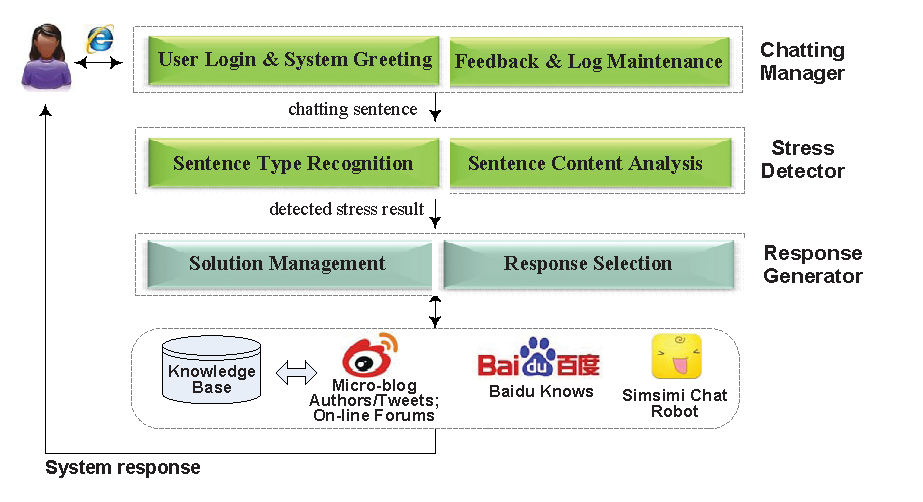
\includegraphics[height=4.9cm]{figs/TeenChatterFramework.eps}
\caption{\emph{TeenChat} framework}
\label{fig:framework}
\end{figure}

\emph{TeenChat} works under the Browser/Server mode. Fig.~\ref{fig:framework} shows its
framework. The user chats with \emph{TeenChat} via an Internet browser.
The \emph{TeenChat} server is comprised of three major components,
which cooperate as follows.
\begin{itemize}
\item \textbf{Chatting Manager}. After a user logins to the system, the \emph{User Login}\&\emph{Sys}
\emph{tem Greeting} module
sends a warm greeting to the user based on the historically detected stress result.
If no historic stress is detected, \emph{TeenChat} will send a greeting like a virtual friend
``\emph{Hello, how��s doing?}", or ``\emph{Is everything ok now}?".
if the user had some stress being detected through previous conversations,
The \emph{Feedback}\&\emph{Log Maintenance} module maintains and refreshes the detected stress result, and adjusts the response
strategy based on feedback analysis (i.e., whether the chatting lasts long, whether the answers
is effective to alleviate user's stress, etc.)

\item \textbf{Stress Detector}.
To understand user's expected answer from the system, the \emph{Sentence Type Recognition} module
categorizes user's chatting sentence into \emph{interrogative question}, \emph{rhetorical question}, or \emph{declarative sentence}.
An interrogative question sentence like ``\emph{How to improve
maths?}" or \emph{What shall I do?}" may ask for objective or positive answers/suggestions,
while a rhetorical question sentence like ``\emph{They should know me, shouldn't they?}"
may reflect user's certain emotions to some extent.
Furthermore, the \emph{Sentence Content Analysis} module senses user's possible stress, including stress category and stress subcategory,
based on the seven adolescent's stress-related lexicons.
If the user's stress is sensed but no stress category/subcategory can be detected
from the current chatting sentence, the previous or historic stress category/subcategory (if available) is assumed as the current stress category/subcategory.
The working of the \emph{Sentence Content Analysis} module is detailed in the next section.


\item  \textbf{Response Generation}.
Based on the stress detection result as well as the chatting sentence type, the
\emph{Response Selection} module chooses an appropriate answer from the local Knowledge Base, Baidu Knows,
or the existing chatting robot Simsimi Repository~\cite{30SIMSIMI}.
The aim is to help stressful users shift attention or express inner struggling, thus
easing the pressure.
The \emph{Solution Management} module is responsible for setting up \emph{TeenChat}'s response strategies during chatting,
and pre-storing a large volume of positive answering sentences in
a local knowledge base, to be managed and incrementally populated
by crawling from on-line forums and influential micro-blog authors/tweets.
\end{itemize}

\section{Stress Detection}
From a user's input sentence $c$, \emph{TeenChat} firstly tries to sense whether the user has some stress or not
based on our stress-related emotion lexicon in Table 1.
Meanwhile, it builds a linguistic dependency tree for $c$, whose root node is the core
word of the sentence.
\emph{TeenChat} analyzes all possible linkage between the stress emotion word and stress category/sub-category words in the tree,
and returns a set of triples of the form:
\texttt{(Stress, Category:$l_c$, SubCategory:$l_s$)},
where \texttt{Stress} takes value 0 (meaning no stress detected) or 1 (meaning stress detected),
$l_c$ is the path length between the negative emotional word and the category node,
and $l_s$ is the path length between the negative emotional word and the sub-category node.
$l_c$/$l_s$ can be null if there exists no path linking the negative emotion word and
the category/sub-category word.
\begin{table}
\label{tab:lexicons}
\begin{minipage}{\textwidth}
\centering
\caption{Stress-Related Lexicons}

\begin{tabular}{ll|l} \\ \hline
\multicolumn{3}{l}{\textbf{I. Stress Emotion Lexicon}} \\ \hline
\multicolumn{2}{l|}{Negative Emotion} & \emph{stress, stressful, pressure,  nervous, unhappy, annoyed,} \\
  &      & \emph{annoying, bad, sad, etc.} \\ \hline
\multicolumn{2}{l|}{Positive Emotion} & \emph{happy, relaxed, good, fun, etc.} \\ \hline
\multicolumn{2}{l|}{Negation}  & \emph{no, not, neither, etc.} \\ \hline

\multicolumn{3}{l}{\textbf{II. Stress Category/Sub-Category Lexicon}} \\ \hline
STUDY & Homework & \emph{homework, project, practice, assignment, etc.} \\ \cline{2-3}
      & Exam     & \emph{exam, grade, mark, rank, score, etc.} \\ \cline{2-3}
      & General  & \emph{history, math, physical, etc.}  \\ \hline
SELF-      & Appearance & \emph{ugly, fat, stout, etc.} \\ \cline{2-3}
COGNITION      & Health     & \emph{sleepless, flustered, insomnia, fracture, stomachache, etc.} \\ \cline{2-3}
& Inner-feeling & \emph{foolish, stupid, awkward, incapable, self-distrust, etc.} \\ \cline{2-3}
               & General & \emph{unconfident, inferior, abased, weak, etc.} \\ \hline
INTER- & Family & \emph{father, mother, brother, sister, uncle, aunt, etc.} \\\cline{2-3}
PERSONAL & Teacher & \emph{teacher, school, regulation, schoolmaster, etc.} \\ \cline{2-3}
& Friend & \emph{classmate, friendship, etc.} \\ \cline{2-3}
& General & \emph{quarrel, criticize, ridicule, etc.} \\ \hline
AFFECTION & Lover  &  \emph{boyfriend, girlfriend etc.}  \\ \cline{2-3}
  & Partner    &  \emph{partner, etc.}    \\ \cline{2-3}
& General & \emph{break-up, separate, secret-love, unrequited love, etc.} \\ \hline
GENERAL & \multicolumn{2}{l}{(unknown category and sub-category)}   \\ \hline
\end{tabular}
\end{minipage}
\end{table}

\begin{example}
Take sentence ``\emph{Always quarrelling with friends at school, so annoyed!}"  for example.
Fig.~\ref{fig:dependenceTree} gives its linguistic dependency tree, constructed by the
linguistic analysis tool LTP~\cite{Che10}.
The stress-related negative emotion word ``\emph{annoyed}" is linked to
``\emph{quarrel}" via a 1-length path, and to
``\emph{friend}" via a 3-length path.
As ``\emph{quarrel}" belongs to stress category INTER-PERSONAL,
and ``\emph{friend}" to its sub-category Friend, a user's stress in INTER-PERSONAL,
in particular in the Friend aspect, is sensed from the sentence, denoted
as \texttt{(1, INTER-PERSONAL:1, Friend:3)}.
%\boxend
\end{example}

In case multiple stress categories/sub-categories are sensed,
the one with the shortest path between the negative emotion word and
the stress category or sub-category word is considered as the primary stress category/sub-category.
When the path length cannot help make distinction, the category similar to the
historic stress category will be taken as the primary one.
If the above also fails, the primary one is randomly determined.
In this way, from each user's input sentence $c$, a detection result
\texttt{(c.Stress, c.Category, c.SubCategory)} is returned, where
\texttt{c.Stress=0} indicates no stress is discovered from the current sentence $c$, and
\texttt{c.Category/c.SubCategory=null} indicates no category/sub-category word is found in $c$.

Considering user's short dialogue inputs, as well as the consecutiveness of stressful emotion remaining
during conversation, we keep and refresh user's historic stress status,
(\texttt{(h.Stress, h.Category, h.SubCategory)}) detected from the previous sentences as follows. \\
\noindent (1) When no stress is detected from the current sentence $c$, but detected from the history,
if \texttt{h.Category==c.Category} and
\texttt{h.SubCategory==c.SubCategory},\\we mark \texttt{c.Stress=1}. \\
\noindent (2) When stress is detected from the current sentence $c$ with a concrete category/
sub-category, which
is/are missing from the history, we assign \\
\texttt{h.Category=c.Category} and \texttt{h.SubCategory=c.SubCategory}.
\begin{figure}
\makeatletter\def\@captype{figure}\makeatother
\begin{minipage}{.51\textwidth}
\centering
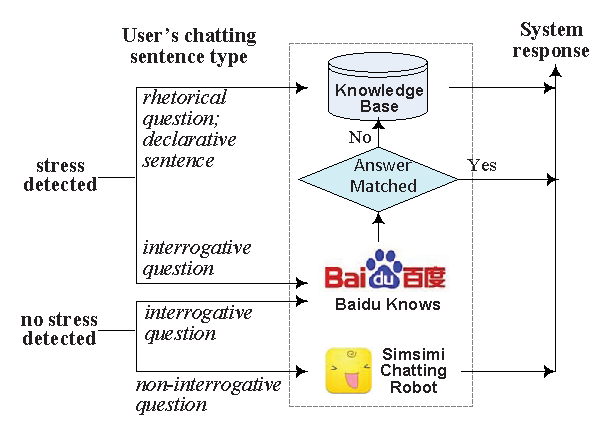
\includegraphics[height=3.5cm]{figs/ResponseStrategy.eps}
\caption{\emph{TeenChat} response strategies}
\label{fig:ResponseStrategy}
\end{minipage}
\makeatletter\def\@captype{figure}\makeatother
\begin{minipage}{.45\textwidth}
\centering
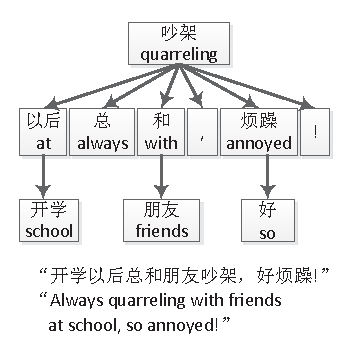
\includegraphics[height=3.5cm]{figs/dependenceTreeExample.eps}
\caption{A dependence tree example}
\label{fig:dependenceTree}
\end{minipage}
\end{figure}

\section{Response Generation Module}

Fig.~\ref{fig:ResponseStrategy} gives \emph{TeenChat}'s response strategies
based on  user's sentence type and the detected result \texttt{(c.Stress,c.Category, c.SubCategory)}.

\noindent [\textbf{Case 1}] Stress being detected (\texttt{c.Stress==1})

\noindent (1) For a user's \texttt{declarative sentence} or \texttt{rhetorical question}, \emph{TeenChat} selects an answer from the \emph{local knowledge base}, which accommodates abundant of positive response sentences in different categories/sub-categories to comfort, encourage, or guide stressful users.

\noindent (2) For a user's \texttt{interrogative question}, \emph{TeenChat} goes to one of the largest Chinese Q\&A community \emph{Baidu Knows} to match the question with the given answer. Let $Q_u$ be the user's input question, and $Q_b$ be the closest question found in the Baidu Knows. If their matching degree $MatchDegree(Q_u,Q_b)$ is over a certain threshold $\theta$, and meanwhile $Q_b$'s corresponding answer has been adopted or agreed by at least one person, \emph{TeenChat} will return $Q_b$'s best answer to the user. Otherwise, \emph{TeenChat} will search the \emph{local knowledge base} and return a general positive answer, or just a joke to cheer up the user.
\begin{figure}
\begin{minipage}{\textwidth}
\centering
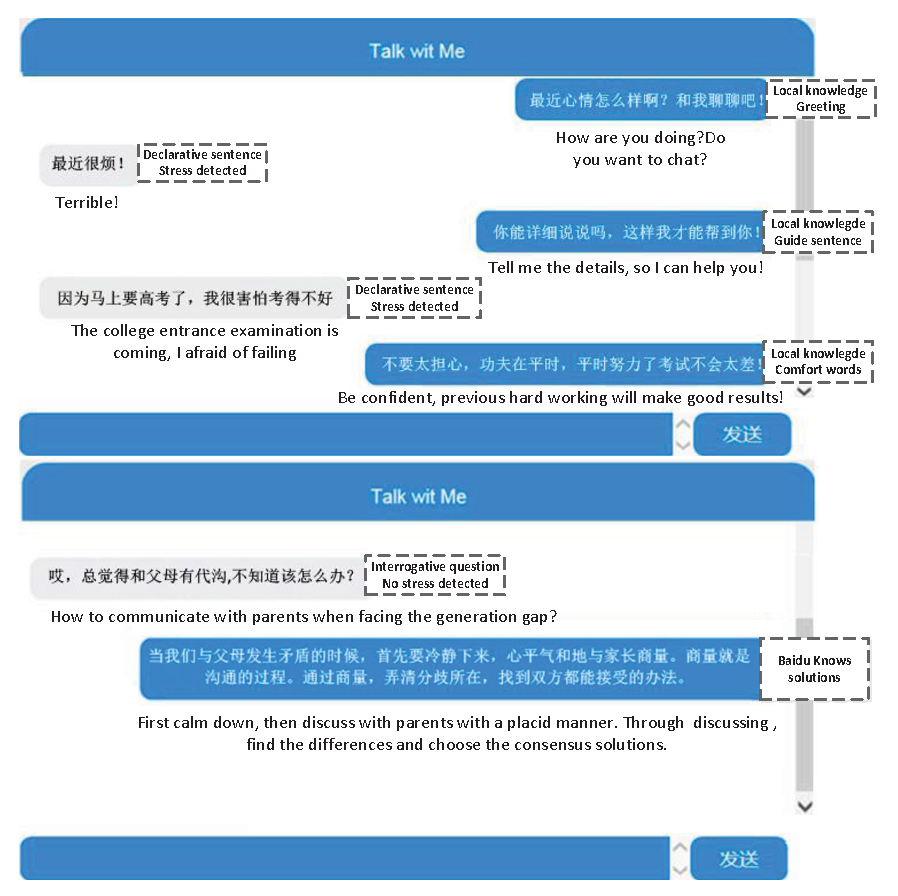
\includegraphics[height=8.8cm]{figs/Dialogexample.eps}
\caption{\emph{TeenChat} response examples of two topic categories}
\end{minipage}
\label{fig:example}
\end{figure}
The matching degree $MatchDegree$$(Q_u$,$Q_b)$ is computed based on the \emph{effective
node pairs} in the $Q_u$'s and $Q_b$'s linguistic dependence trees~\cite{36li2003}.
An \emph{effective node pair} is a node pair $(n_1,n_2)$, where $n_1$ is the core root node, $n_2$ is the direct child node of $n_1$, and $n_2$ represents a verb, noun, or adjective word. Given two effective node pairs $u=(u_1,u_2)$ and $b=(b_1,b_2)$, we define their similarity as:
\[sim(u,b)=sim((u_1,u_2),(b_1,b_2)) = \left\{ \begin{array}{ll}
1   & \mbox{if $(u_1==b_1) \wedge (u_2==b_2)$} \\
0.5 & \mbox{else if $(u_1==b_1) \wedge (u_2 \neq b_2)$} \\
0   & \mbox{otherwise}
\end{array}
\right. \]

Let $E(Q_u)$ and $E(Q_b)$ denote the set of effective node pairs in the $Q_u$'s and $Q_b$'s linguistic dependence trees, respectively.
Considering nodes' semantical equivalence, we replace any two nodes (one in $E(Q_u)$ and the other in $E(Q_b)$) with their
sememe in Hownet (if existing) to ensure nodes' similarity as much as possible. The obtained equivalent effective node sets are denoted as $E^*(Q_u)$ and $E^*(Q_b)$, respectively.
We have
$MatchDegree(Q_u,Q_b)=$
$\alpha ~ SIM(E(Q_u),E(Q_b))+$
$(1-\alpha) ~ SIM(E^*(Q_u),E^*(Q_b))$,
where $\alpha=0.5$,\\
$SIM(E(Q_u),E(Q_b))=\frac{\sum_{u \in E(Q_u)}~\sum_{b \in E(Q_b)}~sim(u,b)}{Max \{|E(Q_u)|, |E(Q_b)|\}}$, and \\
$SIM(E^*(Q_u),E^*(Q_b))=\frac{\sum_{u^* \in E^*(Q_u)}~\sum_{b^* \in E^*(Q_b)}~sim(u^*,b^*)}{Max \{|E^*(Q_u)|, |E^*(Q_b)|\}}$.

\noindent [\textbf{Case 2}] No stress being detected (\texttt{c.Stress==0})

\noindent (1) For a user's \texttt{interrogative question}, the answering is the same as the one in \emph{Case 1} (2).

\noindent (2) For a user's \texttt{non-interrogative question} input, \emph{TeenChat} goes to the open Simsimi repository~\cite{30SIMSIMI}, which provides public API for developers to establish their own chatting robot.

Fig.$4$ shows some example responses about study and interpersonal skills.


\section{User Study }
\subsection{Experimental Setup}
We invited 10 students (aged between 15 and 22) from a high school and a university to participate in our 1-month study. We chose these students because the  majority of the adolescent group are students and the selected students were suffering from more or less stress, as evidenced by their Cohen's Perceived Stress Scale (CPSS-14) results~\cite{SC1983}, which is commonly used to measure human stress level worldwide in psychology. To begin with, the users were told that \emph{Teenchat} was a chatting system which could help them release stress and they could chat with \emph{Teenchat} whenever necessary. During the experiment, we asked the users to do the following things: 1) Fill in the Chinese CPSS questionnaire every week to record the change of their stress status. 2) Evaluate the releasing effect of each conversation. 3) Give the ground truth to the stress status of each sentence in the conversation.
\subsection{Experimental Results}
After the 1-month user study, we obtained: 1) 62 conversations and 1063 chatting sentences in all, namely 6.2 conversations for each user and 17.2 utterances for each conversation in average. 2) 5 Chinese CPSS questionnaires for each user which record their change of  stress status.

\textbf{The accuracy of stress detection. }
 For each conversation, we returned the stress detection result of each sentence to the user and ask the user to judge whether it is right or not. We used the \emph{precision} and \emph{recall} rate to evaluate the accuracy of stress detection. As Table~\ref{tab:stress_detection} showed, the detection of stress existence has a good result with the precision rate of 78.34\% and recall rate of 76.12\%. For the detection of stress category, the recall rate of \emph{affection} and \emph{inter-personal} and the precision rate of \emph{general} are lower than other categories, because some \emph{affection} and \emph{inter-personal} stress are denoted to the \emph{general} stress. Apparently, the stress detection on study, the most common adolescent stress category, has the overall best result with the precision rate of 86.20\% and the recall rate  of 75.00\%.
 
\textbf{The effectiveness of stress release. }
We evaluated the effectiveness of stress release from three aspects:

\textit{The evaluation for the releasing effectiveness of each conversation.}
Users were asked to give a mark (1-5: represent feeling worse, not changed, a bit better, better and much better respectively) to evaluate the stress releasing effectiveness of each conversation. Fig.~\ref{fig:score} shows that more than 60\% conversations get a score higher than 2, namely, making the user feel better. And \emph{Teenchat} is more effective in releasing study stress because detection result of study has higher accuracy.

\textit{The change mode of stressful sentence ratio in a conversation.}
For each conversation, we equally divided the whole chatting process into three stages ($early$, $middle$ and $late$) according to time and computed the ratio of stressful sentences in each stage. Then we analyze the change $Change_n$ from one stage $Ratio_n$ to the next stage $Ratio_{n+1} (Change_n=(Ratio_{n+1}-Ratio_n)/Ratio_{n+1})$. We consider $Change_n$ within $\pm10\%$ as stable($\rightarrow$), $Change_n$ more than $10\%$ as ascend($\uparrow$) and $Change_n$ less than $-10\%$ as descend($\downarrow$). The first four change modes of stressful sentence ratio in Table~\ref{tab:changemode}, denoted by column 2 and column3, mean that \emph{TeenChat} is effective  and the next five change modes mean that \emph{TeenChat} is ineffective. As  Table~\ref{tab:changemode} showed, column 4 reports the frequency of conversations that satisfy the corresponding change mode and the percentage is shown in column 5. Column 6 and 7 report the sum of frequency and percentage of effective and ineffective conversations respectively.
\begin{figure}
\makeatletter\def\@captype{figure}\makeatother
\begin{minipage}{.51\textwidth}
\centering
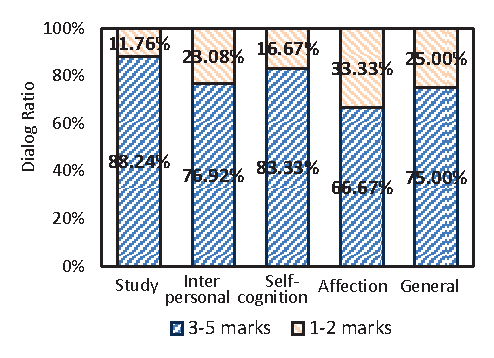
\includegraphics[width=5.5cm]{figs/experimentresult.eps}
\caption{5 stress categories mark distribution}
\label{fig:score}
\end{minipage}
\makeatletter\def\@captype{table}\makeatother
\begin{minipage}{.45\textwidth}
\centering
\caption{Accuracy of stress detection}
\begin{tabular}{c|c|c}
\hline
 &Precision&Recall
\\\hline
 \multicolumn{3}{l}{Accuracy of stress existence detection}
\\\hline
Stress &73.15\%&63.37\%
\\\hline
No stress&83.53\%&88.87\%
\\\hline
Average&78.34\%&76.12\%
\\\hline
 \multicolumn{3}{l}{Accuracy of stress category detection}
\\\hline
Study&86.20\%&75.00\%
\\\hline
Self-Cognition&93.90\%&46.27\%
\\\hline
Inter-Personal&53.84\%&76.56\%
\\\hline
Affection&82.05\%&42.60\%
\\\hline
General&30.94\%&76.92\%
\\\hline
Average&69.39\%&63.47\%
\\\hline
\end{tabular}
\label{tab:stress_detection}
\end{minipage}
\end{figure}
\begin{table}
 \caption{Conversation distribution  of the change mode about stressful sentence ratio}
\centering
\begin{tabular}{c|c|c|c|c|c|c}
\hline
&\multicolumn{2}{|c|}{Change mode}&Freq&Perc&Freq\_sum&Perc\_sum
\\\cline{2-3}
%\\\hline
 &Early-Middle &Middle-Late  &&&&
\\\hline
 &$\downarrow$&$\downarrow$&17&27.42\%&&
\\\cline{2-5}
Effective&$\rightarrow$&$\downarrow$&7&11.29\%&&
\\\cline{2-5}
&$\uparrow$&$\downarrow$&8&12.90\%&45&72.58\%
\\\cline{2-5}
&$\downarrow$&$\rightarrow$&13&20.97\%&&
\\\hline
&$\downarrow$&$\uparrow$&7&11.29\%&&
\\\cline{2-5}
&$\rightarrow$&$\uparrow$&0&0.00\%&&
\\\cline{2-5}
Ineffective&$\rightarrow$&$\rightarrow$&6&9.68\%&17&27.42\%
\\\cline{2-5}
&$\uparrow$&$\rightarrow$&3&4.84\%&&
\\\cline{2-5}
&$\uparrow$&$\uparrow$&1&1.61\%&&
\\\hline
\end{tabular}
%}
\label{tab:changemode}
\end{table}

\textit{The change of users stress status according to Chinese CPSS.}
\begin{table}
 \caption{Number of people of 3 kinds of stress status evolving type}
\centering
\begin{tabular}{c|c|c|c|c}
\hline
 &Improved&Not change&Deteriorated&Total
\\\hline
 Week 1&2&0&8&10
\\\hline
Week 2&5&1&4&10
\\\hline
Week 3&5&1&4&10
\\\hline
Week 4&7&1&2&10
\\\hline
\end{tabular}
\label{tab:CPSS}
\end{table}
For each user, we asked them to fill the Chinese CPSS questionnaire to record the evolving of their stress status. In the questionnaire, higher score represents heavier stress. We consider that score decreasing means the stress status has been improved, score increasing means the stress status has deteriorated. Table~\ref{tab:CPSS} shows that more and more users were feeling better as time goes by.

\section{conclusion}
In this paper, we present an intelligent chatting system for sensing and releasing adolescents' stress. First, we built seven stress-related lexicons and used the natural language processing techniques to sense adolescents' stress. Then we designed the response strategies to act like a virtual friend to listen, comfort, encourage and understand the stressful adolescents to help release stress. Our user study showed a good result of \emph{TeenChat} in stress detection and stress release. In our future work, we will make use of abundant resources in social network to improve the response effect, including collecting more answers with higher pertinency and efficiency. Then another direction we will consider is how to further solve the privacy problem of chatting processing.\\
\section*{Acknowledgement. }
The work is supported by National Natural Science Foundation of China (6137
3022, 61370023, 61073004), and Chinese Major State Basic Research Development 973 Program (2011CB302203-2).


\bibliographystyle{abbrv}
\footnotesize
\bibliography{HIS2015-Ref}

\end{document}
